\chapter{Practice: Publishing data in Cosm}

Create a user in \emph{\color{blue}{\href{http://cosm.com}{Cosm.com}}} .
You will receive an email with a pointer to create an API-Key.
Create this key as you will need it to interact with cosm.

\begin{lstlisting} [caption = {Command to create a feed}, language = sh, label = {code:create-feed}, numbers = left, escapeinside={@}{@}]

curl --request POST \
     --data '{"title":"My feed", "version":"1.0.0"}' \
     --header "X-ApiKey: YOUR_API_KEY_HERE" \
     --verbose \
     http://api.cosm.com/v2/feeds

\end{lstlisting}

Use the API Key you obtained in the previous step.
Next edit a JSON file (name it, for example, cosm.json) with the contents detailed in Listing \ref{code:data-json}.

Observe the output as in Fig. \ref{fig:create-feed} and you will observe a feed id (the last number in the Location line).

\begin{figure}[htbp]
  \centering
  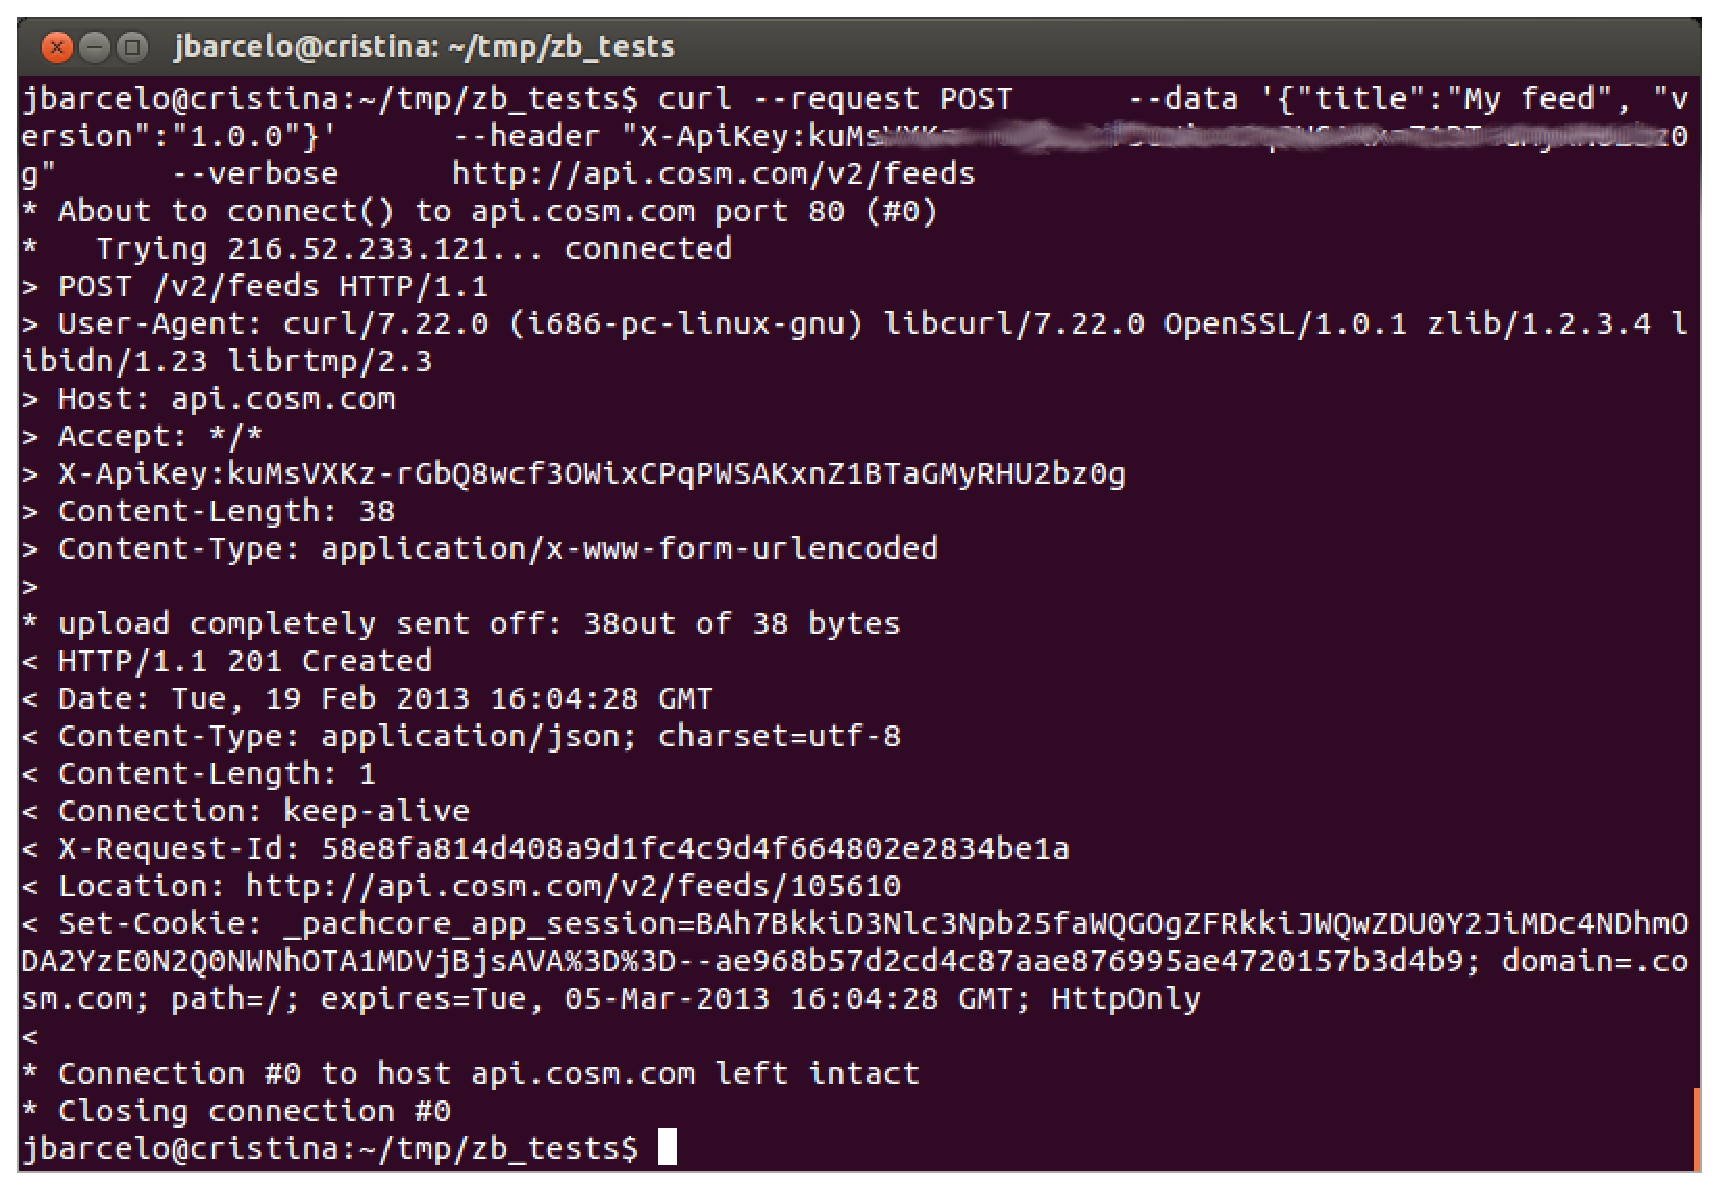
\includegraphics[width=0.9\linewidth]{figures/create-feed.eps}
  \caption{Creating a feed in COSM using curl}
  \label{fig:create-feed}
\end{figure}

Create a JSON file with some dummy data to update to Cosm as in Listing \ref{code:data-json}.

\begin{lstlisting} [caption = {JSON file with data to be uploaded to Cosm}, language = sh, label = {code:data-json}, numbers = left, escapeinside={@}{@}]
{
  "version":"1.0.0",
  "datastreams":[
      {"id":"0", "current_value":"100"},
      {"id":"two", "current_value":"500"},
      {"id":"3.0", "current_value":"300"}
  ]
}
\end{lstlisting}

And now you can update the data to Cosm using the curl command.

\begin{lstlisting} [caption = {Command to upload data to a feed}, language = sh, label = {code:uploading}, numbers = left, escapeinside={@}{@}]
curl --request PUT \
     --data-binary @cosm.json \
     --header "X-ApiKey: YOUR-API-KEY-HERE" \
     --verbose \
     http://api.cosm.com/v2/feeds/YOUR-FEED-ID
\end{lstlisting}

And if we look on Cosm's web interface, we should be able to see some beautiful plots as in Fig. \ref{fig:plots}

\begin{figure}[htbp]
  \centering
  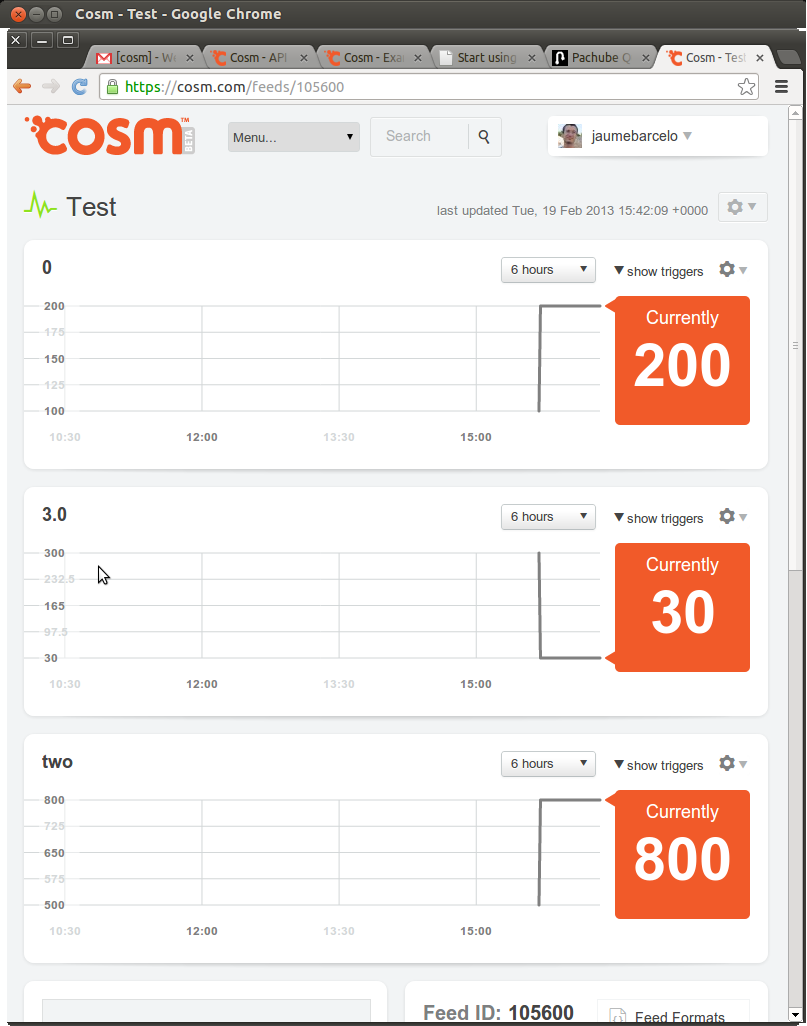
\includegraphics[width=0.9\linewidth]{figures/plots.eps}
  \caption{Plotting data}
  \label{fig:plots}
\end{figure}

You can also read data from the command line as exemplified in Fig. \ref{fig:reading-cosm}.

\begin{figure}[htbp]
  \centering
  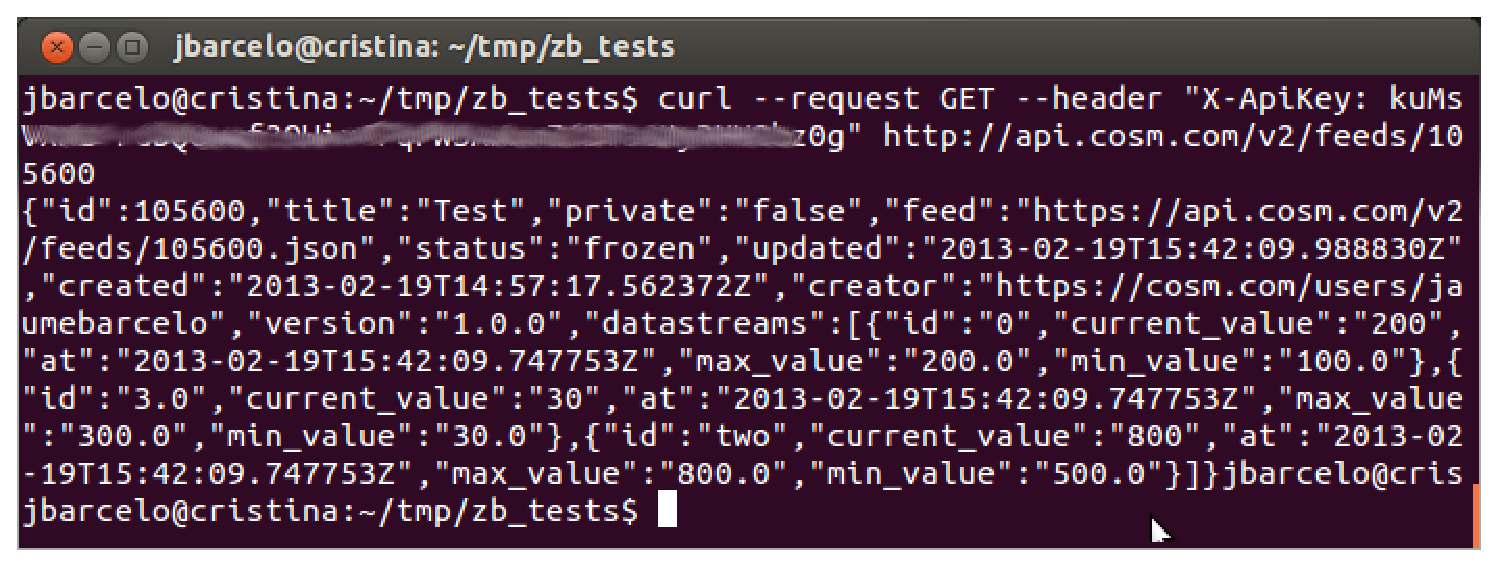
\includegraphics[width=0.9\linewidth]{figures/reading-cosm.eps}
  \caption{Reading a Cosm feed from the command line}
  \label{fig:reading-cosm}
\end{figure}

The next step is to gather information from an XBee and publish it in Cosm.
Use the code detailed in Listing \ref{code:XBee2COSM} as a reference.

\begin{lstlisting} [caption = {Command to upload data to a feed}, language = python, label = {code:XBee2COSM}, numbers = left, escapeinside={@}{@}]
# Derived from code by Alejandro Andreu
import commands
import json
import serial
import time
from serial import SerialException
from xbee import ZigBee

print 'Asynchronously printing data from remote XBee'

serial-port = serial.Serial('/dev/ttyUSB0', 9600)

def print-data(data):
    """
    This method is called whenever data is received.
    Its only argument is the data within the frame.
    """
    print data['samples'][0].keys()[0]

    # Create a JSON file and fill it with the received samples
    json-data = {}
    json-data['version'] = '0.2'
    json-data['datastreams'] = ()
    json-data['datastreams'] = json-data['datastreams'] + ({'id': data['samples'][0].keys()[0], 'current-value': str(data['samples'][0].values()[0])},)
    # Add more datastreams if needed
    with open('cosm.json', mode='w') as f:
        json.dump(json-data, f, indent = 4)
    # Upload information to COSM. Use your own Api Key and feed identifier
    commands.getstatusoutput('curl ... write the curl command here')

zigbee = ZigBee(serial-port, callback = print-data)

time.sleep(1)

zigbee.halt();
serial-port.close()
\end{lstlisting}

Now you can pursue more challenging goals.
For example:
\begin{itemize}
\item Gather information from multiple sensors in a node.
\item Gather information from multiple nodes.
\item Transform the measures of the temperature sensor to Celsius degrees.
\end{itemize}

